\documentclass[10pt]{article}
\usepackage[spanish]{babel}
\usepackage{natbib}
\usepackage{url}
\usepackage{bm}
\usepackage[spanish]{babel}
\usepackage[utf8]{inputenc}
\usepackage{siunitx}
%\usepackage[utf8x]{inputenc}
\usepackage{amsmath}
\usepackage{graphicx}
\usepackage{parskip}
\usepackage{fancyhdr}
\usepackage{amsmath}
\usepackage{caption}
\captionsetup{justification=centering,singlelinecheck=false}
\usepackage{vmargin}
\usepackage{anyfontsize}
\usepackage{enumitem}
\usepackage{xcolor}
\usepackage{cancel}
\usepackage{setspace}
\usepackage{hyperref}
\usepackage{multicol}
\usepackage{subfigure}
\usepackage{pgfplots}
\graphicspath{{../img/}}
\setmarginsrb{2.5 cm}{2 cm}{2.5 cm}{2 cm}{0.8 cm}{1 cm}{.8 cm}{1 cm}

\title{Transistor TBJ}	            % Titulo del trabajo.
\author{Del Rio, Francisco}
\date{\vspace{-5ex}}
\newcommand{\materia}{Dispositivos semiconductores(86.03)}
\newcommand{\padron}{110761}     
\newcommand{\mail}{ fadelrio@fi.uba.ar}

\makeatletter
\let\thetitle\@title
\let\theauthor\@author
\makeatother

\pagestyle{fancy}
\fancyhf{}
\rhead{\theauthor|\padron}
\lhead{
\includegraphics[height=1cm]{resources/logo_fiuba.png}}
\chead{\large\materia \\ \normalsize\thetitle}
\cfoot{\thepage}

\begin{document}
\title{\textbf{\underline{Dispositivos semiconductores (86.03)} \\
Trabajo Práctico N°2: Transistor TBJ}}
\maketitle

%%%%%%%%%%%%%%%%%%%%%%%%%%%%%%%%%%%%%%%%%%%%%%%%%%%%%%%%%%%%%%%%%%%%%%%%%%%%%%%%%%%%%%%

\section{Obtención de las curvas características}
\quad Realicé dos simulaciones con el transistor PNP 2SAR372P5; en la primera (fig. \ref{fig:simulacion_salida}) $I_B$ se mantenía constante mientras que $V_{CE}$ variaba entre \si{-4}{V} y \si{0}{V}, de ésta se obtuvo $I_C$ respecto a $V_{CE}$; en la segunda (fig. \ref{fig:simulacion_transferencia}) se mantenía constante $V_{CE}$ mientras que $V_{BE}$ variaba entre \si{-0,8}{V} y \si{-0,4}{V}, de ésta obtuve $I_C$ e $I_B$ respecto a $V_{BE}$. Para ambas simulaciones se supone una temperatura de 300K Los gráficos de las curvas obtenidas se encuentran en la próxima sección, junto a los ajustes necesarios.
\begin{figure}[ht!]
\begin{minipage}{.5\textwidth}
\centering
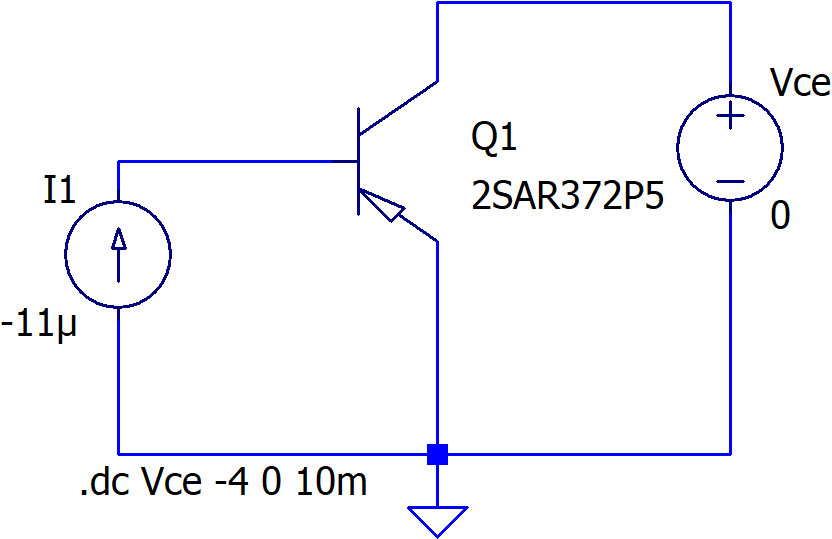
\includegraphics[width=0.6\linewidth]{resources/simulacion_salida.png}
\caption{Circuito para curva de salida}
\label{fig:simulacion_salida}
\end{minipage}
\begin{minipage}{.5\textwidth}
\centering
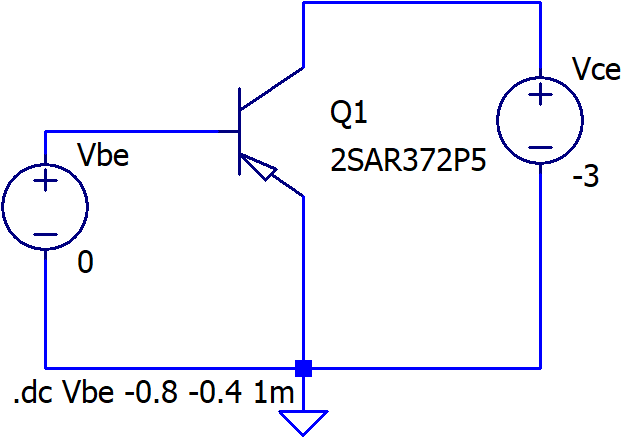
\includegraphics[width=0.6\linewidth]{resources/simulacion_transferencia.png}
\caption{Circuito para curva de transferencia}
\label{fig:simulacion_transferencia}
\end{minipage}
\end{figure}

%%%%%%%%%%%%%%%%%%%%%%%%%%%%%%%%%%%%%%%%%%%%%%%%%%%%%%%%%%%%%%%%%%%%%%%%%%%%%%%%%%%%%%%

\section{Obtención de parámetros característicos}

\quad Utilizando las ecuaciones \ref{eq:1} y \ref{eq:2} y ajustes mediante un software numérico (GNU Octave), obtuve valores de $\beta$, $I_S$, $V_A$ y $V_{CE_{sat}}$. A continuación se detallan los ajustes realizados. 

\begin{equation}\label{eq:1}
    i_{c}=-I_{S} exp \left( \frac{-V_{BE}}{V_{Th}}\right)\left(1+\frac{-V_{CE}}{V_A}\right)
\end{equation}

\begin{equation}\label{eq:2}
    i_c = \beta i_B
\end{equation}

\subsection{Curvas características}

\begin{figure}[ht!]
\begin{minipage}{.5\textwidth}
\centering
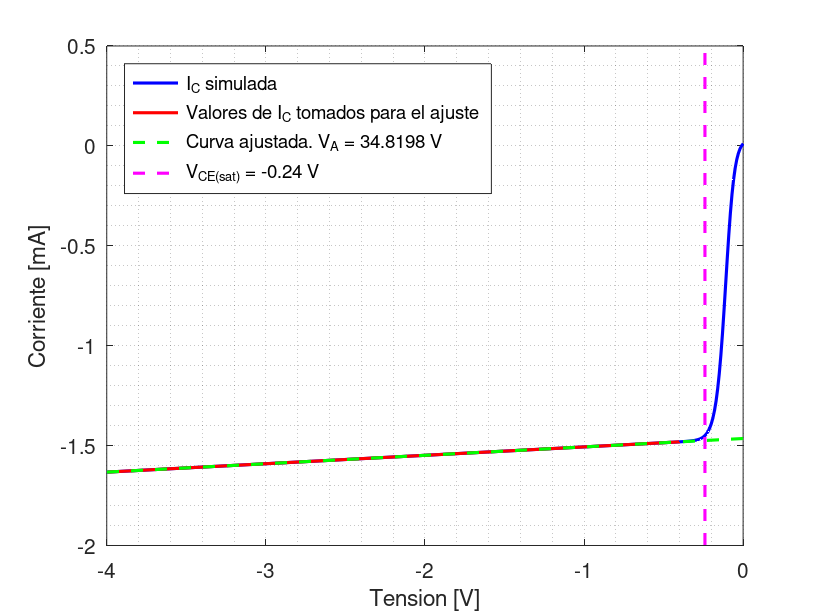
\includegraphics[width=1.1\linewidth]{resources/grafico_curva_de_salida.png}
\caption{Curva de salida con sus respectivos ajustes}
\label{fig:grafico_curva_de_salida}
\end{minipage}
\begin{minipage}{.5\textwidth}
\centering
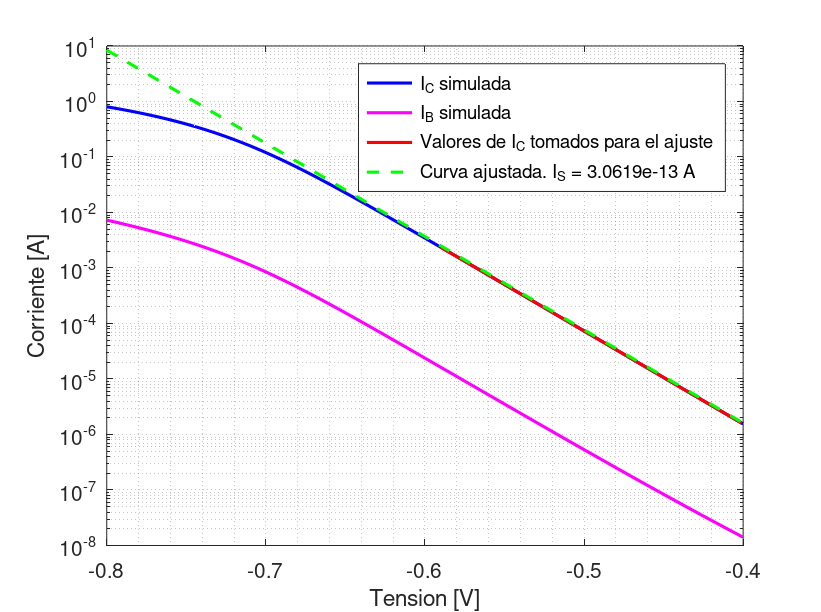
\includegraphics[width=1.1\linewidth]{resources/grafico_curva_transferencia.png}
\caption{Curva de transferencia con sus respectivos ajustes}
\label{fig:grafico_curva_de_transferencia}
\end{minipage}
\end{figure}


\quad Para la curva de salida (fig. \ref{fig:grafico_curva_de_salida}), la cual grafiqué en escala lineal, realicé un ajuste de orden 1 en la zona de modo activo directo, con el fin de obtener $V_A$, cuyo valor es la abscisa al origen de la recta obtenida mediante el ajuste. El valor de $V_A$ obtenido es de \si{34,8198}{V}. Además, de la curva de salida, esta vez mediante un ajuste visual, obtuve un valor aproximado para $V_{CE_{(sat)}}$ el cual se encuentra en el cambio de modo de operación del transistor (entre saturación y M.A.D). El valor de $V_{CE_{(sat)}}$ obtenido es de \si{-0,24}{V}.

\quad Para la curva de transferencia (fig. \ref{fig:grafico_curva_de_transferencia}), la cual grafiqué en escala semilogarítmica, también realicé un ajuste de orden 1, con el fin de obtener $I_S$. Para este caso, se depreció el efecto early, ya que de esta forma la corriente dependerá solo de $V_{BE}$ (eq. \ref{eq:1}); y se utilizaron valores de $V_{BE}$ para los cuales la pendiente de la recta ajustada era similar a $V_{Th}^{-1}$. El valor obtenido de $I_S$ es de \si{306,19}{fA}.

\subsection{Obtención de $\beta$}

\quad El último gráfico a ajustar es el de $\beta$, la relación entre $i_C$ e $i_B$, para el cual utilicé un ajuste de orden 0, tomando los valores de $V_{BE}$ para los cuales el gráfico era más similar a una función constante. El valor obtenido de $\beta$ es de \si{145,2212}.

\begin{figure}[ht!]
    \centering
    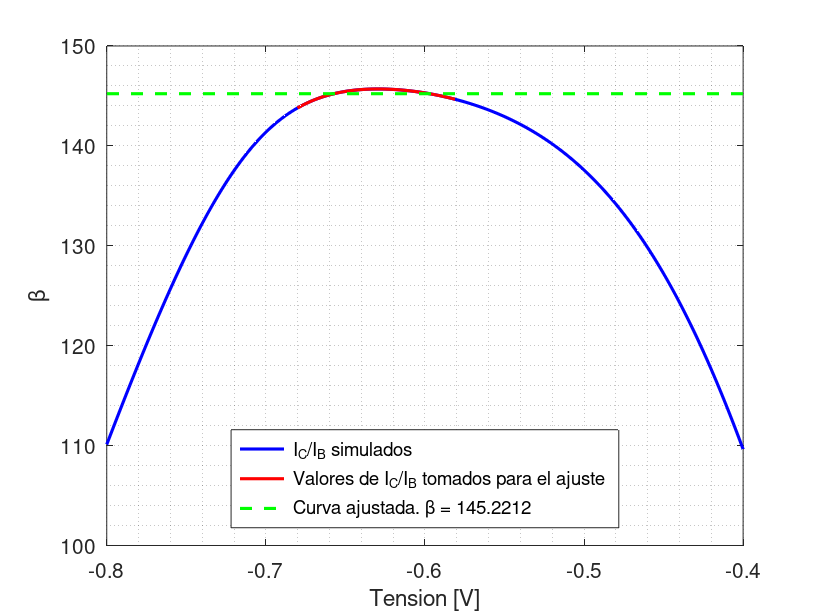
\includegraphics[width=0.5\linewidth]{resources/grafico_beta.png}
    \caption{$\beta$ respeto a $V_{BE}$}
    \label{fig:grafico_beta}
\end{figure}



\section{Información de los fabricantes}
\quad El principal fabricante del transistor utilizado es Rohm Semiconductor, los datos utilizados para comparar los obtenidos mediante los ajustes son los proporcionados por la hoja de datos que se encuentra en la página oficial\footnote{https://www.rohm.com/products/transistors/bipolar-transistors/standard-bipolar-transistors/2sar372p5-product} del fabricante. A continuación se presenta una tabla con todos los datos.

\begin{table}[ht!]
  \begin{center}
    \caption{Resultados obtenidos al resolver utilizando los distintos modelos}
    \label{tab:cuadrode_resultados}  %etiqueta para referenciar la tabla
    \begin{tabular}{|l|l|l|} % cantidad de columnas que va a tener representadas por las letras l, c, r, que indican el alineamiento (left, center, right). Una barra vertical "|" entre dos letras representa una linea dibujada entre las dos columnas
    \hline
      Parámetro & Valor ajustado & Hoja de datos\\ 
      \hline
      $\beta$ & \si{145,2212} & \si{120}-\si{390} \\
      \hline        %este comando entre dos filas, agrega una línea que las separa
      $I_S$ & \si{306,19}{fA} & \si{425,79}{fA} \\
      \hline
      $V_A$ & \si{34,8198}{V} & \si{41,6}{V} \\ 
      \hline
      $V_{CE_{(sat)}}$ & \si{-0,24}{V} & \si{-180}{mV} Typ. \si{-360}{mV} Max. \\
      \hline
    \end{tabular}
  \end{center}
  
\end{table}
\quad Los valores de $I_S$ y $V_A$ fueron obtenidos mediante un ajuste visual de los gráficos proporcionados en las Fig. 1 y 2 de la hoja de datos. Cabe destacar que las curvas utilizadas para obtener estos valores no se correspondían exactamente a los parámetros utilizados para obtener los datos obtenidos mediante el ajuste de las simulaciones, en el caso de $I_S$, la curva de la hoja de datos se correspondía a una temperatura de \si{298,15}{K}, y el el caso de $V_A$, la curva utilizada de la hoja de datos se correspondía a $I_B = $ \si{-0,2}{mA}. Debido a lo mencionado, no se plantea el error relativo en la tabla, ya que las fuentes de error exceden a el error posible de la simulación.

\section{Polarización del transistor}

\begin{figure}[ht!]
    \centering
    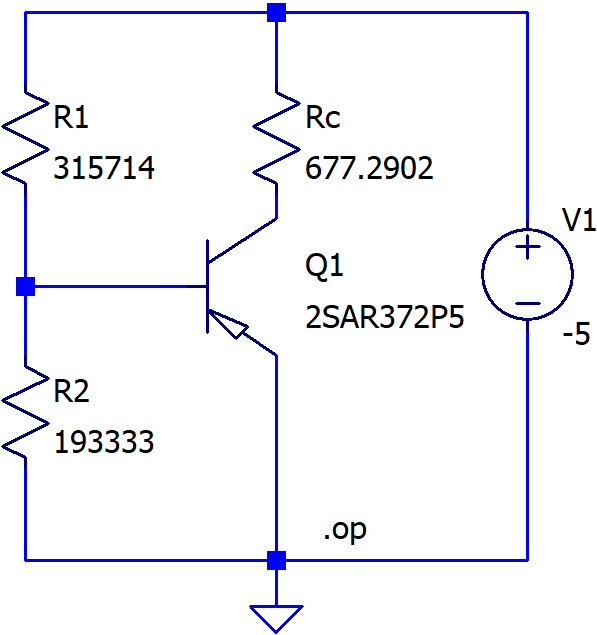
\includegraphics[width= 0.35\linewidth]{resources/simulacion_polarizacion.png}
    \caption{Circuito a analizar, representado en LTSpice}
    \label{fig:simulacion_polarizacion}
\end{figure}

\quad Para la polarización del transistor, donde los datos conocidos son $V_A$, $\beta$, $I_B=$ \si{-11\mu}{A} y $V_{CE}=$ \si{-3,8}{V}, comencé planteando ecuaciones de mallas (eq. \ref{malla_1}, \ref{malla_2}, \ref{malla_3}) y de el nodo que une $R_1$, $R_2$ y la base del transistor (eq. \ref{nodo_alfa}).

\begin{multicols}{2}
  \noindent\begin{equation}
  \label{malla_1}
    -I_C R_C - V_{CE} -\si{5}{V} = 0
  \end{equation}
  \begin{equation}
  \label{malla_2}
    -I_2 R_2 + V_{BE} = 0
  \end{equation}
\end{multicols}
\begin{multicols}{2}
  \noindent\begin{equation}
  \label{malla_3}
    -I_C R_C - V_{BC} +I_1 R_1 = 0
  \end{equation}
  \begin{equation}
  \label{nodo_alfa}
    I_1-I_B-I_2 = 0
  \end{equation}
\end{multicols}

\quad Como el valor de $V_{CE}$ se encuentra en el rango para el cual el transistor opera en M.A.D, vale que 

\begin{equation}
    I_C = \beta I_B \left(1-\frac{V_{CE}}{V_A}\right)
\end{equation}

 entonces, $I_C$ resulta \si{-1,7718}{mA}. Conociendo $I_C$, y mediante un muy simple despeje, resulta evidente que $R_C=$ \si{677,2902\Omega}. Luego, despejando $R_1$ de \ref{malla_3} y $R_2$ de \ref{malla_2}
 
\begin{multicols}{2}
  \noindent\begin{equation}
  \label{r_1}
    R_1 = \frac{I_C R_C - V_{BC}}{I_1}
  \end{equation}
  \begin{equation}
  \label{r_2}
    R_2 = \frac{V_{BE}}{I_2}
  \end{equation}
\end{multicols}

\quad Si bien $V_{BE}$ no es dato, gracias a la curva de la fig. \ref{fig:grafico_curva_de_transferencia} y el dato de $I_B$, $V_{BE}$ resulta \si{-0,58}{V} y luego, como $V_{BC} = V_{BE}-V_{CE}$, $V_{BC}$ resulta \si{3,22}{V}. Como el sistema de ecuaciones del circuito resulta compatible indeterminado, planteo una solución para la cual $I_1 = $ \si{-14\mu}{A}. Luego, reemplazando en \ref{r_1} y \ref{r_2} con los datos obtenidos, resulta $R_1 = $ \si{315,714k\Omega} y $R_2 = $ \si{193,333k\Omega}. Finalmente, ya que $I_E = -I_C -I_B$, resulta $I_E = $ \si{1,7828m}{A}.
\quad Por ultimo, con los valores de resistencias obtenidos, simulé el circuito con el software LTSpice. En la siguiente tabla se comparan los datos obtenidos analíticamente con los obtenidos por simulación


\begin{table}[ht!]
  \begin{center}
    \caption{Comparación de resultados analíticos con los simulados}
    \label{tab:cuadro_comparativo_de_resultados}  %etiqueta para referenciar la tabla
    \begin{tabular}{|l|l|l|l|} % cantidad de columnas que va a tener representadas por las letras l, c, r, que indican el alineamiento (left, center, right). Una barra vertical "|" entre dos letras representa una linea dibujada entre las dos columnas
    \hline
      Parámetro & Resultado analítico & Simulación & Error relativo\\ 
      \hline
      $I_C$ & \si{-1,7718}{mA} & \si{-1,6287}{mA} & 0,08\\
      \hline        %este comando entre dos filas, agrega una línea que las separa
      $I_E$ & \si{1,7828m}{A} & \si{1,6397m}{A} & 0,08\\
      \hline
      $V_{BE}$ & \si{-0,58}{V} & \si{-0,5797}{V} & 0,0004\\ 
      \hline
      $V_{CE}$ & \si{-3,8}{V}  & \si{-3,896}{V} & 0,02\\
      \hline
      $V_{BC}$ & \si{3,22}{V} & \si{3,317}{V} & 0,03\\
      \hline
      $I_{1}$ & \si{-14\mu}{A} & \si{-14\mu}{A} & 0\\
      \hline
      $I_{2}$ & \si{-3\mu}{A} & \si{-2,9989\mu}{A} & 0,0004 \\
      \hline
    \end{tabular}
  \end{center}
  
\end{table}

\section{Análisis de resultados}

\quad Sobre los datos obtenidos mediante ajustes de las curvas características del transistor, comparando con los datos proporcionados por el fabricante, en cuanto a los valores de $\beta$ y $V_{CE_{(sat)}}$, ambos se encuentran dentro del rango mencionado en la hoja de datos, por lo que se pueden considerar a estos valores correteos. Sin embargo, para $I_S$ y $V_A$ no se puede hacer la misma afirmación con tanta seguridad, ya que estos datos no se proporcionan explícitamente en la hoja de datos, si no que se tuvieron que obtener mediante un ajuste precario de los gráficos proporcionados por el fabricante, que tampoco cumplían exactamente con los parámetros de base utilizados en las simulaciones de este informe. Por esto es que si bien los errores relativos no son catastróficos (0,28 para $I_s$ y 0,16 para $V_A$) sería incorrecto darle algún valor, mas allá de lo anecdótico, a los errores obtenidos.

\quad Otro aspecto que vale la pena mencionar es que, como se puede observar en la fig. \ref{fig:grafico_curva_de_transferencia}, la ecuación \ref{eq:1},  despreciando el efecto early, resulta una buena aproximación para valores entre \si{-0,64}{V} y \si{-0,4}{V}, presentando un error absoluto de 10 para \si{-0,8}{V}.
 
\quad Por otro lado, en los  cálculos de polarización del transistor, basta con una breve mirada a la tabla \ref{tab:cuadro_comparativo_de_resultados} para darse cuenta que los resultados obtenidos poseen una alta exactitud en cuanto a lo simulado, el error máximo que se aprecia es de un 8\%. Que si bien por si solo no significa mucho, ya que el error soportado depende íntimamente del contexto en el que se lo utilice, considerando que muchos de los parámetros utilizados se obtuvieron mediante aproximaciones (como $\beta$, $V_A$ y $V_{BE}$), y parte de la resolución se basa en un modelo, un error menor al diez por ciento se puede considerar exitoso.

\section{Conclusiones} 

\quad Como ya se mencionó en la sección anterior, aquellos resultados que pueden ser comparados con fuentes externas a este informe (hoja de datos, simulación) se encontraron dentro de margenes de error aceptables, por lo menos para el marco de este trabajo. 

\quad Un aspecto que me gustaría destacar (que no se detalla tanto en este informe, pero aún así lo veo como una consecuencia favorable de este trabajo) es el uso de octave como herramienta de cálculo numérico, ya que como esta vez no se nos proporcionó un script detallado para realizar los ajustes, me vi obligado a entender cómo funciona el ajuste. Resalto el valor de esto ultimo ya que, notando la falta de parámetros como $I_S$ o $V_A$ en las hojas de datos, me siento capaz de obtenerlos por mi cuenta mediante análisis de resultados experimentales.

\quad Al fin y al cabo, este trabajo resultó útil para afianzar los conocimientos sobre los transistores bipolares de juntura, como así familiarizarme con las curvas características de estos.


\end{document}
